Section \ref{sec:challenges-control-rod} highlighted the poor performance of neutron diffusion
methods for calculating neutron fluxes near control rods. Strong neutron absorption in the control
rod region produces highly anisotropic neutron flux extending some distance outside the control
rod. Neutron transport methods, which retain angular dependence of the neutron flux in one way or
other, generally fare better than neutron diffusion methods with isotropic diffusion coefficients.
However, neutron transport methods are also generally more computationally expensive given the
increased dimensionality of the problem from the angular component. Piling this extra dimension on
top of the existing geometric and neutron energy group dimensions greatly multiplies the unknowns
to be solved in a system. Many past efforts have tried introducing transport correction techniques
to improve neutron flux and multiplication factor estimates with diffusion-based methods. Other
than control rod regions, these techniques also correct for homogenization error introduced from
spatial homogenization of fuel assemblies and other structures within a reactor core. They
invariably rely on neutron transport methods to generate transport corrections in the form of
corrected diffusion coefficients, boundary conditions, Eddington factors or discontinuity factors.

In this chapter, I propose a novel hybrid method for improving control rod modeling in neutron
diffusion solvers without spatial homogenization. In essence, the hybrid method involves applying
the $S_N$ discrete ordinates neutron transport method on subregions containing the control rod to
obtain transport corrected diffusion coefficients for the diffusion method on the entire problem
domain. 

Section \ref{sec:hybrid-theory} discusses the theoretical background for the Hybrid $S_N$-Diffusion
method. Thereafter, Section \ref{sec:preliminary} discusses preliminary results of a 1-D hybrid
method implemented with the finite difference method on several example cases based off the
graphite-moderated \gls{MSRE} reactor design.

\section{Theory} \label{sec:hybrid-theory}

The proposed Hybrid $S_N$-Diffusion method is a two-level, iterative method to improve the
accuracy of neutron diffusion solutions in reactor systems with highly neuutron-absorbing control
rod regions. In this discussion, I focus on the 1-D, time-independent implementation of the
hybrid method.

The discrete ordinates ($S_N$) method for solving the multigroup neutron transport equation
(Eq. \ref{eq:mg-bte}) discretizes the continuous angular directional phase space into a finite
number of discrete angular intervals (ordinates). The set of distinct direction variables
$\hat{\Omega}_n$ representing the discrete ordinates is typically chosen in conjunction with a
compatible quadrature set to replace the integrals across the continuous solid angles
$\hat{\Omega}$ with quadrature approximations. The multigroup, discrete ordinates ($S_N$
approximation) form of the 1-D, time-independent neutron transport equation with the Gauss-Legendre
quadrature set is given as:
%
\begin{align}
  \mu_n \frac{d}{dx}\Psi_g(x, \mu_n) + \Sigma_{t,g}(x)&\Psi_g(x, \mu_n) -
\sum^G_{g'=1} \sum^N_{n'=1} \sum^L_{l=0} \frac{\left(2l+1\right)}{2}
\Sigma^{g'\rightarrow g}_{s,l}(x) P_l(\mu_{n'} - \mu_n)
w_{n'}\Psi_{g'}(x,\mu_{n'}) \nonumber \\
  &= \sum^G_{g'=1} \frac{\chi_g}{2} \frac{\nu\Sigma_{f,g}(x)}{k} \phi_{g'}(x) + S_g(x,\mu_n)
  \label{eq:1d-sn}
  \shortintertext{where}
  \mu_n &= \mbox{ cosine of $\hat{\Omega}_n$ relative to the $x$-axis,} \nonumber \\
  \Psi_g(x,\mu_n) &= \mbox{ neutron angular flux along $\mu_n$ in group $g$,} \nonumber \\
%  g &= \mbox{ neutron energy group index, ranging from 1 to G,} \nonumber \\
%  \Sigma_{t,g}(x) &= \mbox{ macroscopic total cross section of neutrons in group $g$,} \nonumber \\
%  G &= \mbox{ total number of energy groups,} \nonumber \\
%  n &= \mbox{ discrete ordinate index,} \nonumber \\
%  N &= \mbox{ total number of discrete ordinates,} \nonumber \\
  l &= \mbox{ Legendre order,} \nonumber \\
  L &= \mbox{ highest Legendre order,} \nonumber \\
  \Sigma^{g'\rightarrow g}_{s,l}(x) &= \mbox{ $l$-th Legendre expansion of the macroscopic
scattering} \nonumber \\
  &\ \ \ \ \mbox{ cross section from group $g'$ to $g$,} \nonumber \\
  P_l &= \mbox{ $l$-th Legendre polynomial,} \nonumber \\
  w_{n'} &= \mbox{ $n'$-th quadrature weight,} \nonumber \\
%  \chi_g &= \mbox{ fission neutron spectrum in group $g$,} \nonumber \\
%  \nu &= \mbox{ neutrons produced per fission reaction,} \nonumber \\
%  \Sigma_{f,g}(x) &= \mbox{ macroscopic fission cross section of neutrons in group $g$,}
%  \nonumber \\
  k &= \mbox{ neutron multiplication factor.} \nonumber
%  \phi_{g'}(x) &= \mbox{ scalar neutron flux in group $g$,} \nonumber \\
%  S_g(x,\mu_n) &= \mbox{ external neutron source in group $g$.} \nonumber
\end{align}
%
The neutron scalar flux and current can be retrieved by calculating the 0th and 1st Legendre moments
as follows:
%
\begin{align}
  \phi_g(x) &= \frac{1}{2} \int^1_{-1} d\mu\ \Psi_g(x,\mu) = \frac{1}{2} \sum^N_{n=1} w_n
\Psi_g(x,\mu_n)
  \shortintertext{and}
  J_g(x) &= \frac{1}{2} \int^1_{-1} d\mu\ \mu\Psi_g(x,\mu) = \frac{1}{2} \sum^N_{n=1} w_n
\mu_n \Psi_g(x,\mu_n)
\end{align}

The 1-D form of the multigroup time-independent neutron diffusion equations (Eq. \ref{eq:mg-diff})
is given as:
%
\begin{align}
  -\frac{d}{dx} D_g(x) \frac{d}{dx} \phi_g(x) + \Sigma_{t,g}(x) \phi_g(x) &= \sum^G_{g'=1}\left[
  \Sigma_s^{g'\rightarrow g}(x)\phi_{g'}(x) + \chi_g\frac{\nu\Sigma_{f,g'}(x)}{k}
  \phi_{g'}(x)\right] + S_g(x)
  \label{eq:1d-diff}
  \shortintertext{where}
    D_g(x) &= \frac{1}{3 \Sigma_{tr}(x)} = \mbox{ neutron diffusion coefficient for group }g.
  \nonumber
\end{align}

\subsection{Spatially Varying Diffusion Coefficients} \label{sec:svdc}

The conventional approach for determining diffusion coefficients based on the $P_1$ approximation
for each subregion involves running a high-fidelity neutron transport to tally region-wide
estimates of the neutron transport cross section. In essence, a single value represents the
isotropic diffusion coefficient for the entire (e.g. fuel, moderator, reflector) subregion.
However, as discussed in Section \ref{sec:challenges-control-rod}, the neutron diffusion equation
is only valid in regions of high scattering-to-absorption ratios and away from interfaces to
neighboring media with highly dissimilar neutronic properties.

In the Hybrid $S_N$-Diffusion method, I propose replacing the conventional $P_1$-based
diffusion coefficients with an alternate formulation which incorporates point-wise corrections
to the neutron diffusion flux solution from the $S_N$-derived flux solution as follows:
%
\begin{align}
  D^s_g(x) &= -J^{tr}_g(x)\bigg/\frac{d\phi^{tr}_g(x)}{dx}. \label{eq:svdc}
\end{align}
%
where $D^s$ is the \glspl{SVDC}, and the $tr$ superscript denotes neutron current and scalar flux
solutions from the $S_N$ method.
The basic form of this equation is Fick's first law of diffusion. The end result is a diffusion
coefficient variable that varies in space even within a subregion and provides pointwise
corrections to closely match the diffusion flux solution to the $S_N$ flux solution.

Pounders \& Rahnema \cite{pounders_diffusion_2009} demonstrated the effectiveness of applying
point-wise corrections derived from analytical or Monte Carlo reference flux solutions. Compared
with conventional $P_1$-based out-scatter and flux-limited approximations of the diffusion
coefficient, their \textit{high-order empirical diffusion coefficient} showed superior agreement
with the reference flux solutions. Their formulation for these piecewise-constant empirical
diffusion coefficients in Eq. \ref{eq:emp} is similar to the formulation for \glspl{SVDC} in Eq.
\ref{eq:svdc} after finite difference discretization. They recognized that the volume
averaging for piecewise-constant coefficients introduce some truncation error if the flux is
non-linear within each mesh element. This design choice may be due to an intention to retain the
diffusion coefficient as a constant in the $\frac{d}{dx}D\frac{d\phi}{dx}$ term of the neutron
diffusion equation (Eq. \ref{eq:1d-diff}).

Unlike their approach, the \gls{SVDC} formulation in Eq. \ref{eq:svdc} allows for continuously
varying diffusion coefficients to reduce truncation error. In practice, the discretization order of
\gls{SVDC} variables in a numerical calculation would follow the discretization order of the
reference flux solution. This formulation introduces a minor change to the finite difference
implementation of the second-order diffusion term to specifically handle spatial derivatives of the
diffusion coefficient, but the finite element implementation sees no change as the second-order
diffusion term is commonly treated with integration-by-parts to reduce it to a first-order
differential term with no derivatives of the diffusion coefficient. Refer to Section
\ref{sec:implementation} for the numerical implementation of a finite difference neutron diffusion
solver with \glspl{SVDC}.

\begin{figure}[htb!]
  \centering
  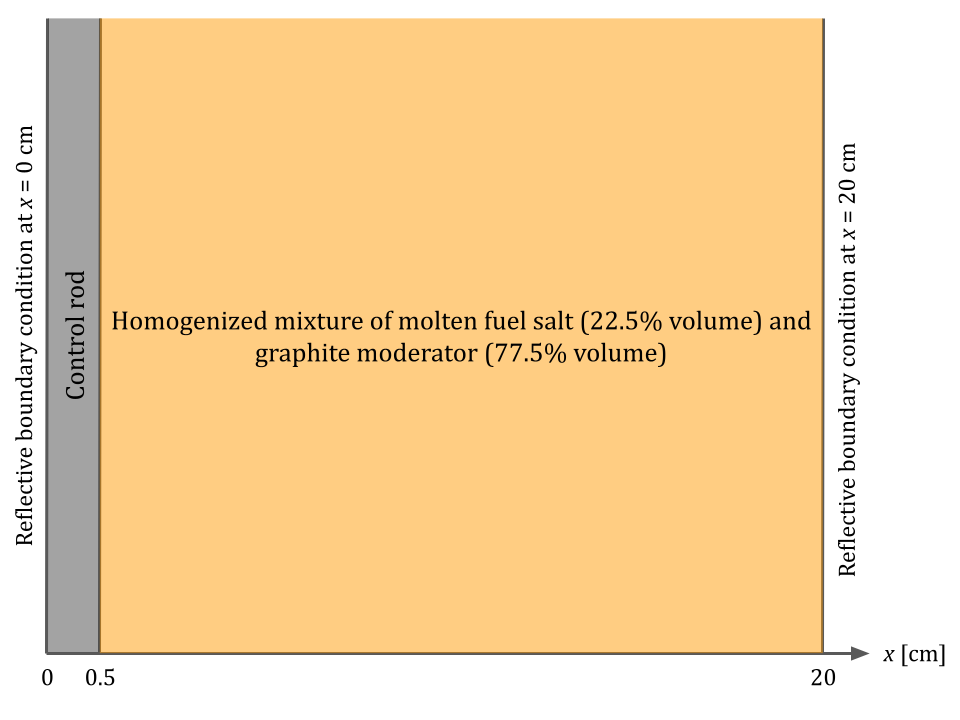
\includegraphics[width=.7\columnwidth]{case-0-geometry}
  \caption{A 1-D, two-region system containing a 0.5 cm-thick control rod and a 24.5 cm-thick
    homogeneous mixture of molten fuel salt and graphite moderator. Reflective boundary conditions
    are applied on both ends.}
  \label{fig:case-0-geom}
\end{figure}

\subsubsection{\gls{SVDC} Verification with Case 0}

To facilitate the following demonstration of a neutron diffusion calculation with \glspl{SVDC},
consider a 1-D, two-region system (Case 0) consisting of a highly neutron absorbing material and a
neutron multiplying region with reflective boundary conditions on both ends (Figure
\ref{fig:case-0-geom}). The material specifications are taken from the control rod, molten fuel
salt, and graphite moderator compositions of the \gls{MSRE} \cite{robertson_msre_1965}. The molten
fuel salt and graphite regions are homogenized to minimize discrepancies arising from geometrical
heterogeneity. The group constant input data for the diffusion and $S_N$ solvers (e.g. cross
sections, fission spectra, etc.) were sampled at 900 K the OpenMC Monte Carlo neutronics software.
The neutron energy spectrum is condensed into two discrete groups bounded at $10^{-5}$, $10^0$, and
$10^8$ eV.

I solved for the neutron flux in this system using the following set of numerical solvers:
%
\begin{enumerate}
  \item Diffusion solver with $P_1$ flux-limited diffusion coefficients generated directly from the
    OpenMC calculation.
  \item $S_4$ solver with up to 1st-order Legendre expansions of the group-to-group neutron
    scattering cross sections.
  \item Diffusion solver with \glspl{SVDC} generated from the prior $S_4$ flux solution.
\end{enumerate}
%
All other relevant group constants are identical and unchanged from the original dataset generated
using OpenMC. I implemented the diffusion solvers using the finite difference method and the $S_N$
solver using a diamond-differenced transport sweep method in the Python programming language. For
brevity, further numerical implementation details of these solvers are deferred to Section
\ref{sec:implementation}.

\begin{figure}[htb!]
  \centering
  \begin{subfigure}[b]{.49\textwidth}
    \centering
    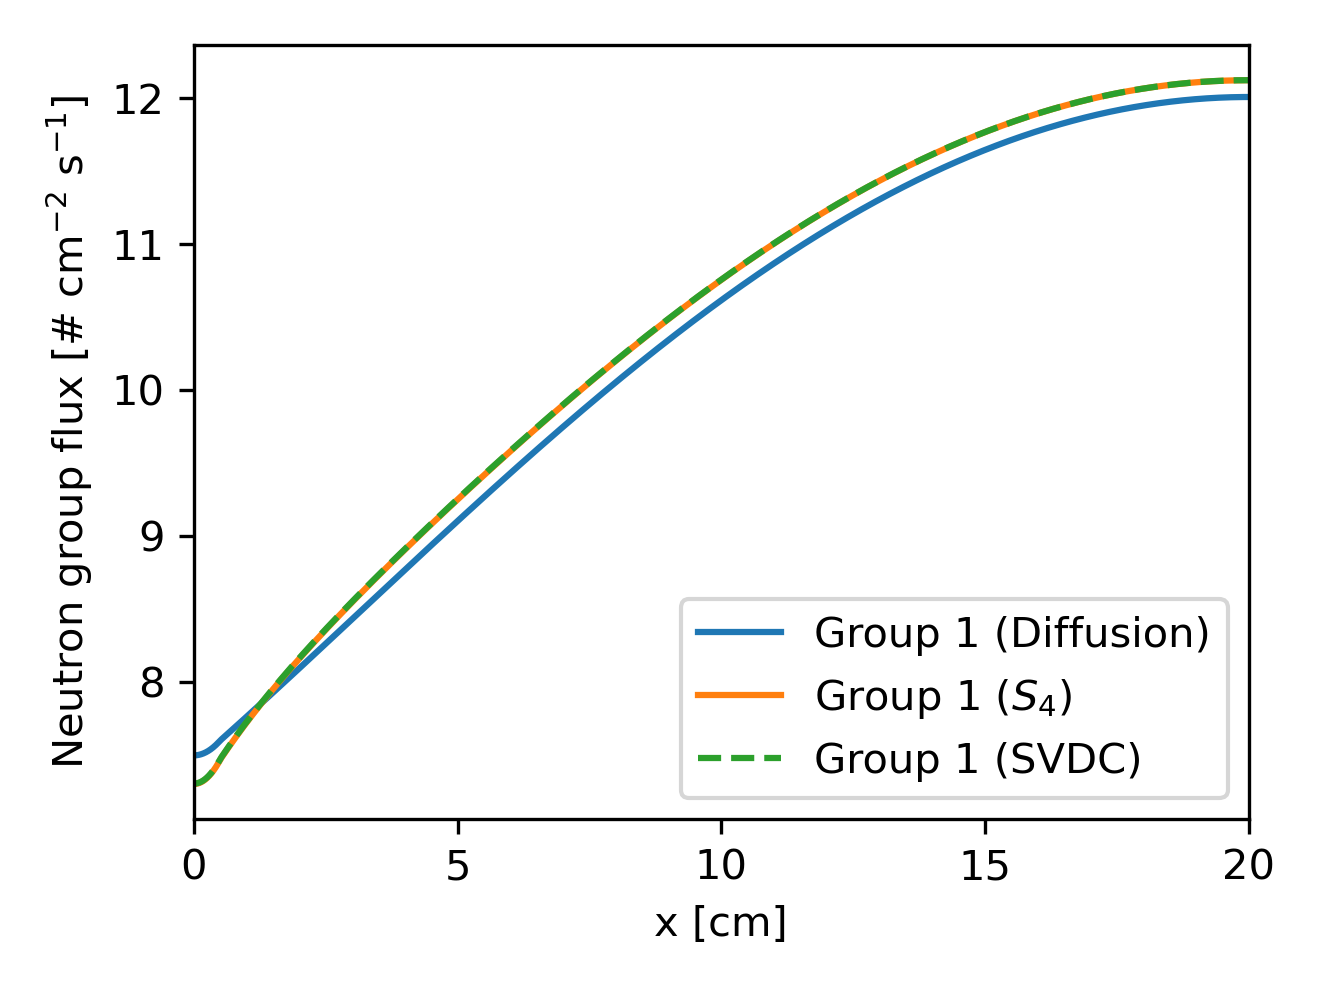
\includegraphics[width=\textwidth]{case-0-group-1-flux}
    \caption{Group 1 flux}
    \label{fig:c0g1flux}
  \end{subfigure}
  \hfill
  \begin{subfigure}[b]{.49\textwidth}
    \centering
    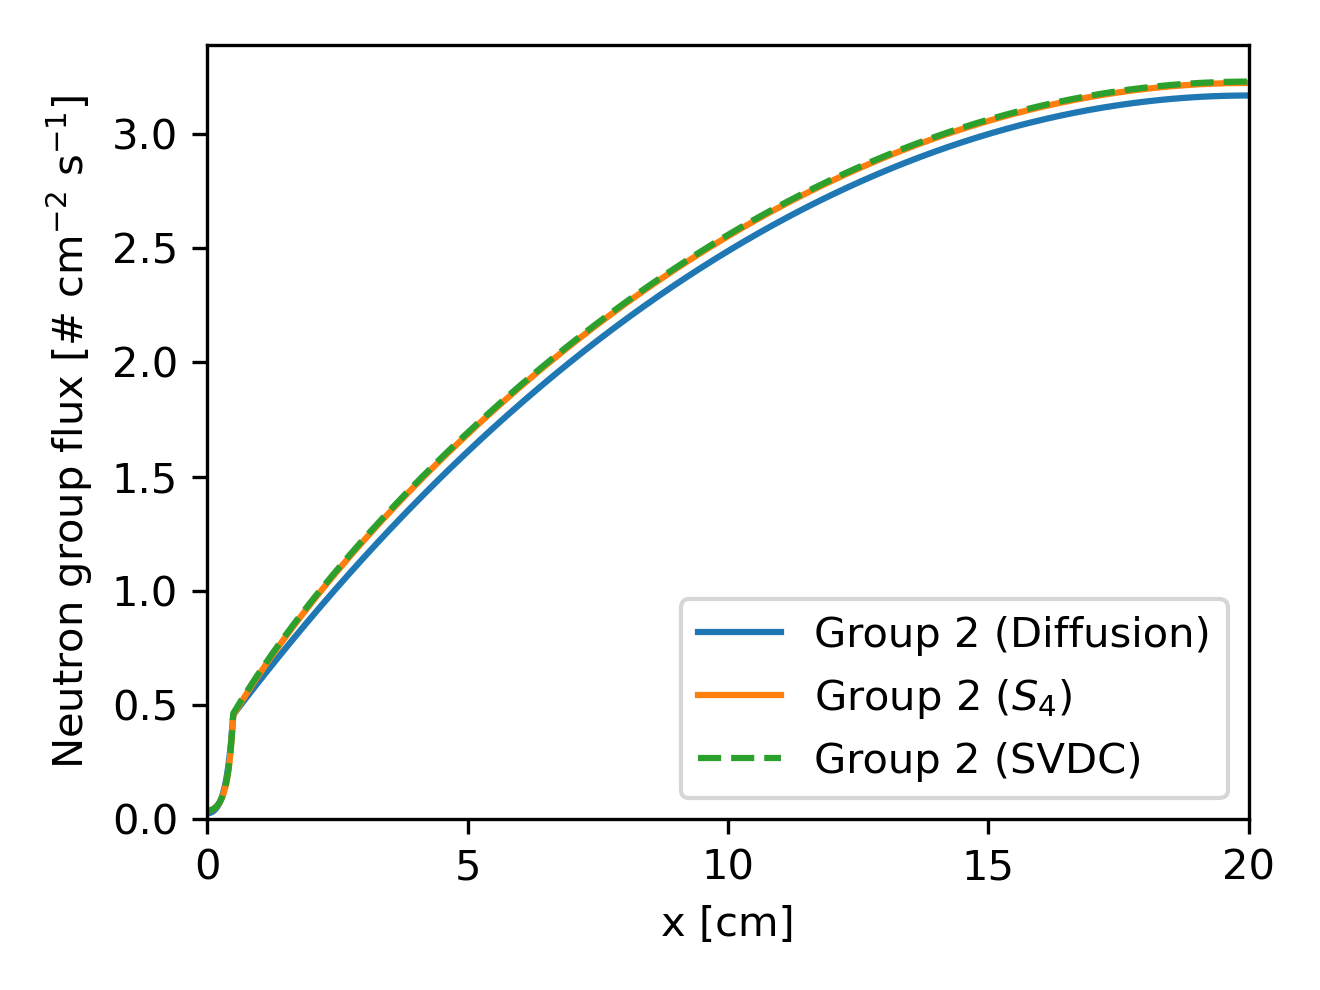
\includegraphics[width=\textwidth]{case-0-group-2-flux}
    \caption{Group 2 flux}
    \label{fig:c0g2flux}
  \end{subfigure}
  \caption{Neutron group 1 and 2 flux distributions from the diffusion, $S_4$, and
  diffusion-\gls{SVDC} solvers for Case 0.}
  \label{fig:c0flux}
\end{figure}
%
\begin{figure}[htb!]
  \centering
  \begin{subfigure}[b]{.49\textwidth}
    \centering
    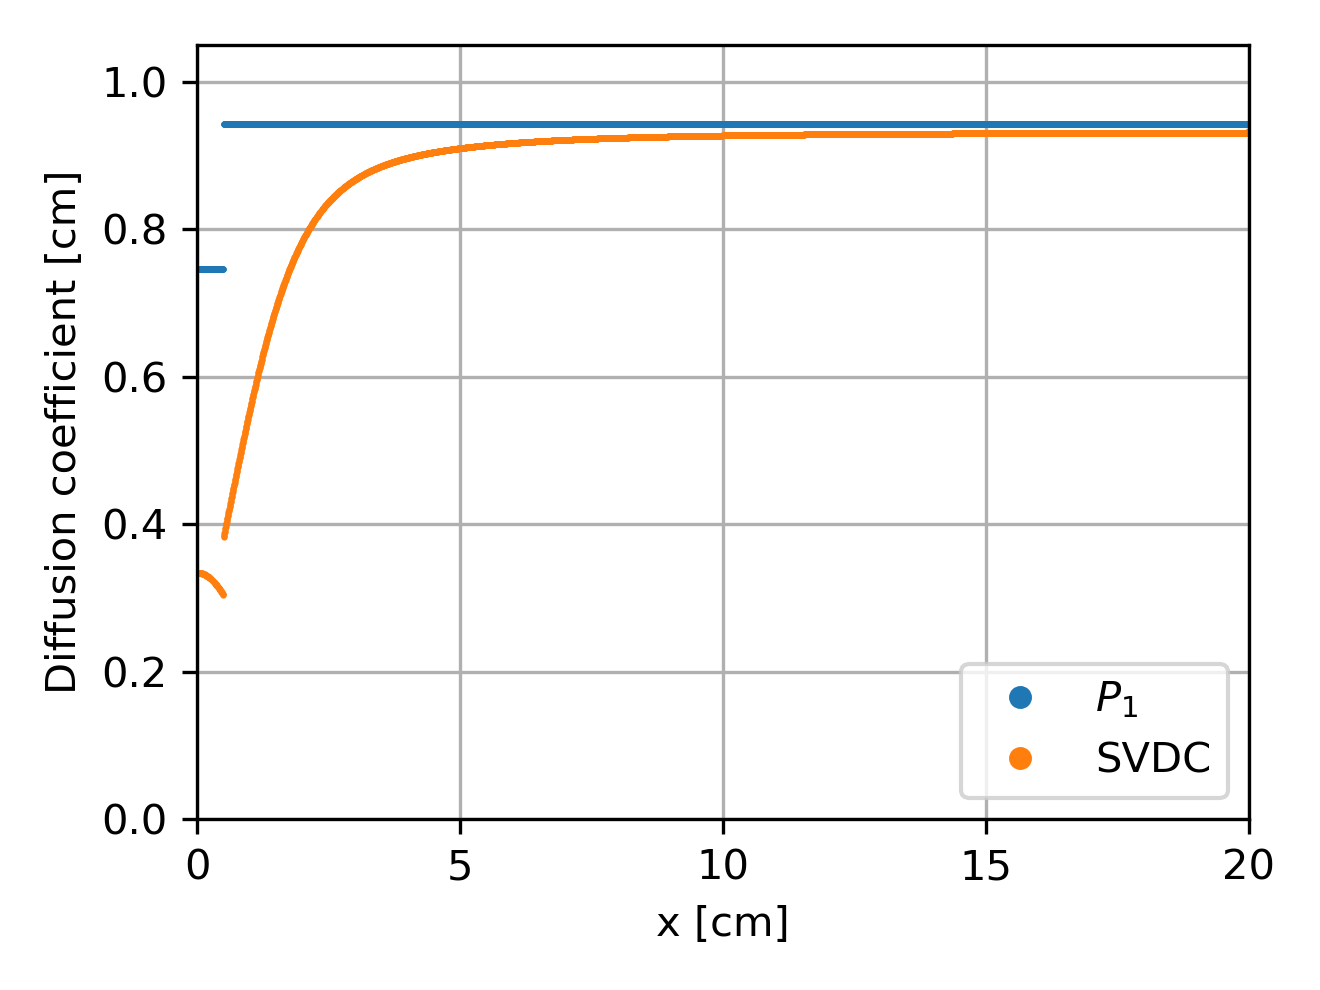
\includegraphics[width=\textwidth]{case-0-group-1-diffcoef}
    \caption{Group 1 diffusion coefficients}
    \label{fig:c0g1diffcoef}
  \end{subfigure}
  \hfill
  \begin{subfigure}[b]{.49\textwidth}
    \centering
    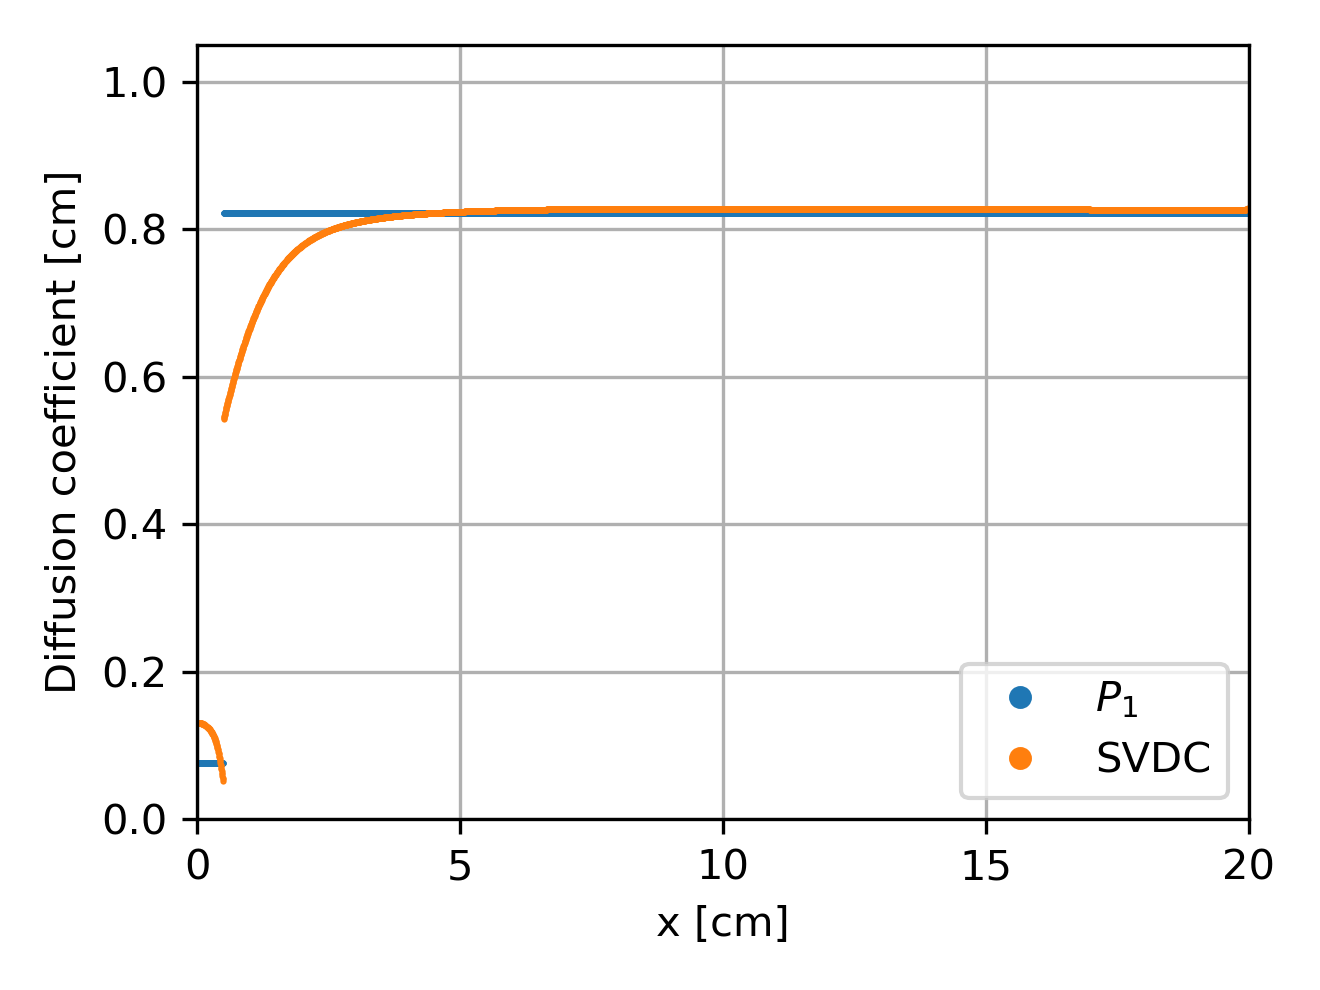
\includegraphics[width=\textwidth]{case-0-group-2-diffcoef}
    \caption{Group 2 diffusion coefficients}
    \label{fig:c0g2diffcoef}
  \end{subfigure}
  \caption{$P_1$-based diffusion coefficient and \gls{SVDC} spatial distributions
  for Case 0.}
  \label{fig:c0diffcoef}
\end{figure}

Figure \ref{fig:c0flux} shows the group 1 and 2 neutron fluxes from the diffusion-$P_1$, $S_4$, and
diffusion-\gls{SVDC} solvers with a fixed mesh size of 0.005 cm. The OpenMC flux solution is
omitted because the purpose of this exercise is to demonstrate the effectiveness of \glspl{SVDC}
in reproducing a $S_N$ flux solution. As expected, the diffusion-$P_1$ flux solution deviates from
the $S_4$ flux solution while the diffusion-\gls{SVDC} flux solution shows significantly better
agreement with the $S_4$ flux solution. As shown in Table \ref{table:c0k}, $k$ estimate from the
diffusion-\gls{SVDC} solver (0.62554) is also closer to the $k$ estimate from the $S_4$ solver
(0.62424) than the diffusion-$P_1$ solver (0.60976).

\begin{table}[tb!]
  \centering
  \caption{Multiplication factor $k$ estimates from the diffusion-$P_1$, $S_4$, and
  diffusion-\gls{SVDC} solvers and the absolute difference relative to the $S_4$ estimate.}
  \begin{tabular}{l S S}
    \toprule
    Solver type & {$k$} & {Diff.} \\
    \midrule
    Diffusion-$P_1$ & 0.60976 & -0.01448 \\
    $S_4$ & 0.62424 & {-} \\
    Diffusion-\gls{SVDC} & 0.62554 & +0.00130 \\
    % OpenMC & {0.64604 +/- 0.00051} & {-} \\
    \bottomrule
  \end{tabular}
  \label{table:c0k}
\end{table}

Comparing the $P_1$-based diffusion coefficients and \glspl{SVDC} in Figure \ref{fig:c0diffcoef},
both quantities agree closely in the bulk fuel salt region far away from the control rod region.
This observation supports the validity of the neutron diffusion method with $P_1$ approximations
in a homogeneous medium with high scattering-to-absorption ratios. Moving towards the control rod
region, the \glspl{SVDC} deviate from the $P_1$-based diffusion coefficients as the prerequisite
assumptions for diffusion theory do not hold anymore.

Another key finding from this study is that the neutron diffusion method with $P_1$-based
diffusion coefficients fails to reproduce the steep $S_4$ flux gradient in the control rod region
for group 1 and in the homogeneous fuel-graphite region adjacent to the control rod region for both
neutron groups. The neutron diffusion method requires small \gls{SVDC} values in those regions to
induce steeper flux gradients and match the $S_4$ flux solution. Given that the presence of highly
neutron-absorbing materials tend to induce steep flux gradients, we can expect similar trends in
the \glspl{SVDC} relative to $P_1$-based diffusion coefficients for other similar systems.

Thus far, this method is trivial and completely redundant because it requires a priori
knowledge of the true flux solution or at least a highly accurate solution calculated using neutron
transport methods. While existing workflows for diffusion-based methods already require
computationally intensive neutron transport simulations to generate input data for the neutron
diffusion equation, this preprocessing step (known as \textit{group constant generation}) requires
a fixed number of neutron transport simulations. For instance, $P_1$-based diffusion coefficients
may be generated at various reactor temperatures. In the subsequent multiphysics reactor analysis,
these diffusion coefficient values may be interpolated for diffusion coefficient estimates at other
temperatures within the validity range. On the other hand, \glspl{SVDC} will likely need to be
dynamically generated at every timestep, such as with a two-level iterative scheme consisting of a
high-level $S_N$ neutron transport calculation and a low-level neutron diffusion calculation.

The nature of \glspl{SVDC} as empirical, pointwise corrections for
the diffusion equation makes it highly dependent on the neutron flux gradient, and
susceptible to greater variations than region-wide estimates for $P_1$-based diffusion
coefficients. Compared to \glspl{SVDC}, $P_1$ diffusion coefficients behave much more like
intrinsic material properties as their definitions are largely tied to material cross sections.
Variations in $P_1$ diffusion coefficients largely arise from changes in the neutron energy
spectrum with no direct contribution from proximity to material interfaces (geometrical
heterogeneity).

Another significant challenge of \glspl{SVDC} and the high-order empirical diffusion coefficients
involves their determination near neutron flux peaks. The neutron currents and
flux gradients in the numerator and denominator of Eq. \ref{eq:svdc} generally do not go to zero at
the same point, resulting in very large positive or negative diffusion coefficient values when the
flux gradient is close or equal to zero. Pounders \& Rahnema tackled this issue by using
larger mesh sizes with which to calculate their empirical diffusion coefficients. However, their
remedy significantly worsens flux accuracy in regions with steep, non-linear flux such as in
control rods. I plan to investigate and find an alternative solution for this issue in the
implementation of \glspl{SVDC} in the proposed work.

\subsection{Hybrid $S_N$-Diffusion Method} \label{sec:hybrid-method}

In order to reduce the computational cost of the high-level $S_N$ calculation, I propose reducing
the problem domain of the $S_N$ method to the control rod and its vicinity. Consequently, this
Hybrid $S_N$-Diffusion method can retain accurate neutron flux estimates around the control rod
region from the $S_N$ method while making significant savings in computational cost by treating the
majority of the reactor geometry with the neutron diffusion method. Henceforth, I will refer to
the $S_N$ calculation or method on the reduced problem domain as the $S_N$ \textit{subproblem} or
\textit{subsolver} accordingly. The problem domains of the neutron diffusion and $S_N$ calculations
are defined as $\Omega^d_0$ and $\Omega^d_1$, respectively, where $\Omega^d_1 \subseteq
\Omega^d_0$. The algorithm for the Hybrid $S_N$-Diffusion method is as follows:
%
%\begin{algorithm}
%  \caption{Hybrid $S_N$-Diffusion algorithm \label{alg:hybrid}}
%  \DontPrintSemicolon
%  \KwData{Material group constants and mesh of problem domain $\Omega^d$.}
%  \KwResult{Improved flux $\phi$ and multiplication factor $k$ estimates.}
%  \BlankLine
%  Initialize $\phi_g^0$, $k^0$, $D_g^0=D_g^{P_1}$; $m=0$\;
%  \While{$\epsilon_\phi > tol_\phi$ or $\epsilon_k > tol_k$}{
%    $m = m+1$\;
%    Solve the neutron diffusion equations for $\phi_g^m$ and $k^m$ using $D_g$ in domain
%    $\Omega^d$.\;
%    Update $\epsilon_\phi = ||\phi_g^m-\phi_g^{m-1}||_2/G/n$ where $G=$ total no. of groups and
%    $n=$ total no. of mesh elements.\;
%    Calculate neutron current boundary conditions along subdomain boundaries $\partial\Omega^d_1$
%    using $\phi_g^m$ and $D_g$, where $\Omega^d_1 \subset \Omega^d$
%  }
%\end{algorithm}
%
\begin{enumerate}
  \item Start with an initial neutron diffusion calculation in $\Omega^d_0$ with conventional $P_1$
    diffusion coefficients and other standard group constants (e.g. neutron cross sections).
  \item Use the neutron diffusion flux estimates in $\Omega^d_1$ and current estimates along
    $\partial \Omega^d_1$ as initial and boundary conditions for the $S_N$ subsolver.
  \item With the $S_N$ subsolver, calculate an improved neutron flux solution in $\Omega^d_1$ which
    contains the control rod region and its immediate vicinity.
  \item Calculate \glspl{SVDC} using the $S_N$ flux solution and Eq. \ref{eq:svdc}.
  \item Pass the \glspl{SVDC} to the neutron diffusion solver to replace the conventional
    $P_1$ diffusion coefficients within the regions that overlap with the $S_N$ solver problem
    domain.
  \item Start a new iteration by running neutron diffusion calculation with the \glspl{SVDC}
    replacing $P_1$ diffusion coefficients in part or all of $\Omega^d_1$.
  \item Pass the iterative neutron diffusion flux and current solutions to the $S_N$ subsolver.
  \item Iterate until convergence is reached by meeting pre-defined convergence tolerance values.
\end{enumerate}

\subsubsection{$S_N$ Subsolver Boundary Conditions \& Dead Zone Assumptions}

The main challenge lies in determining appropriate boundary conditions for the $S_N$ subproblem.
Given that we want to limit the coverage of $\Omega^d_1$ to the control rod region and its
immediate vicinity, the boundaries $\partial\Omega^d_1$ should lie well within $\Omega^d_0$.
However, there is currently no feasible method of generating accurate boundary fluxes for an $S_N$
solver from a neutron diffusion flux solution. In 1-D, the standard $S_N$ method requires N/2
incoming flux boundary parameters per boundary mesh point for the N/2 neutron angular fluxes
flowing into $\Omega^d_1$. The neutron diffusion method can produce at most one independent
incoming flux parameter per mesh point; this parameter is the neutron forward/backward current in
the $P_1$ approximation defined as:
%
\begin{align}
  J_{g,\pm} &= \frac{\phi_g}{4} \mp \frac{D_g}{2}\frac{d\phi_g}{dx}
  \shortintertext{where}
  J_{g,\pm} &= \mbox{ neutron forward/backward current of group }g. \nonumber \\
\end{align}
%
In the absence of additional information, I will assume that all N/2 angular fluxes are equal in
magnitude, i.e. the flux is isotropic throughout the half-sphere pointing into the $S_N$ subproblem
domain. As a consequence, the $S_N$ subsolver yields an inaccurate flux solution.

To resolve this issue, I posit the following hypothesis: \textit{If there exists a highly
neutron-absorbing control rod region within the $S_N$ subproblem domain $\Omega^d_1$ and the $S_N$
subproblem boundary $\partial\Omega^d_1$ lies several neutron mean free paths away from this
region, the \gls{SVDC} values calculated near the control rod region (using the $S_N$ subsolver
with half-sphere isotropic boundary conditions) will tend to the actual flux gradient solution
(using a reference $S_N$ calculation across the entire problem domain $\Omega^d$).} In other words,
suboptimal boundary conditions may induce inaccurate \gls{SVDC} values near the $\partial
\Omega^d_1$ subdomain boundaries, but the \gls{SVDC} values further from $\partial\Omega^d_1$ are
accurate and very weakly dependent on the boundary conditions. These inaccurate \gls{SVDC} values
close to $\Omega^d_1$ may be discarded in favor of the default $P_1$-based diffusion coefficients.
I will refer to the region containing these discarded values as the \textit{dead zone} or
$\Omega^d_2$, where $\Omega^d_2 \subset \Omega^d_1 \subseteq \Omega^d_0$.

\subsubsection{Hybrid Method Verification with Case 0}

Here, we revisit Case 0, the 1-D two-region system described in Section \ref{sec:svdc} (Figure
\ref{fig:case-0-geom}), to test my hypothesis and demonstrate the Hybrid $S_N$-Diffusion method.
I defined $\Omega^d_1$ to span from $x=0$ cm to $x=17.5$ cm. Note that $\Omega^d_1$
is a subdomain of the entire domain spanning from $x=0$ cm to $x=20$ cm.
Once again, the numerical implementation details are deferred to Section \ref{sec:implementation}.

The size of $\Omega^d_2$
is dynamically determined based on the \gls{SVDC} distribution generated at every iteration during
the hybrid method calculation. In the earlier study with \glspl{SVDC}, the \gls{SVDC} distribution
in the homogeneous fuel-graphite region approaches the $P_1$-based diffusion coefficient value as
$x$ is further from the control rod region. Therefore, starting from the control rod and
fuel-graphite region interface and sweeping right, I set the cutoff point for the $\Omega^d_2$ to
be \textit{the point at which the \gls{SVDC} distribution approaches within 1\% of the $P_1$-based
diffusion coefficient value}. The hybrid method converged after two outer iterations comprising of
three neutron diffusion and two $S_4$ calculations in total as outlined by the hybrid method
algorithm.
%
\begin{figure}[htb!]
  \centering
  \begin{subfigure}[b]{.49\textwidth}
    \centering
    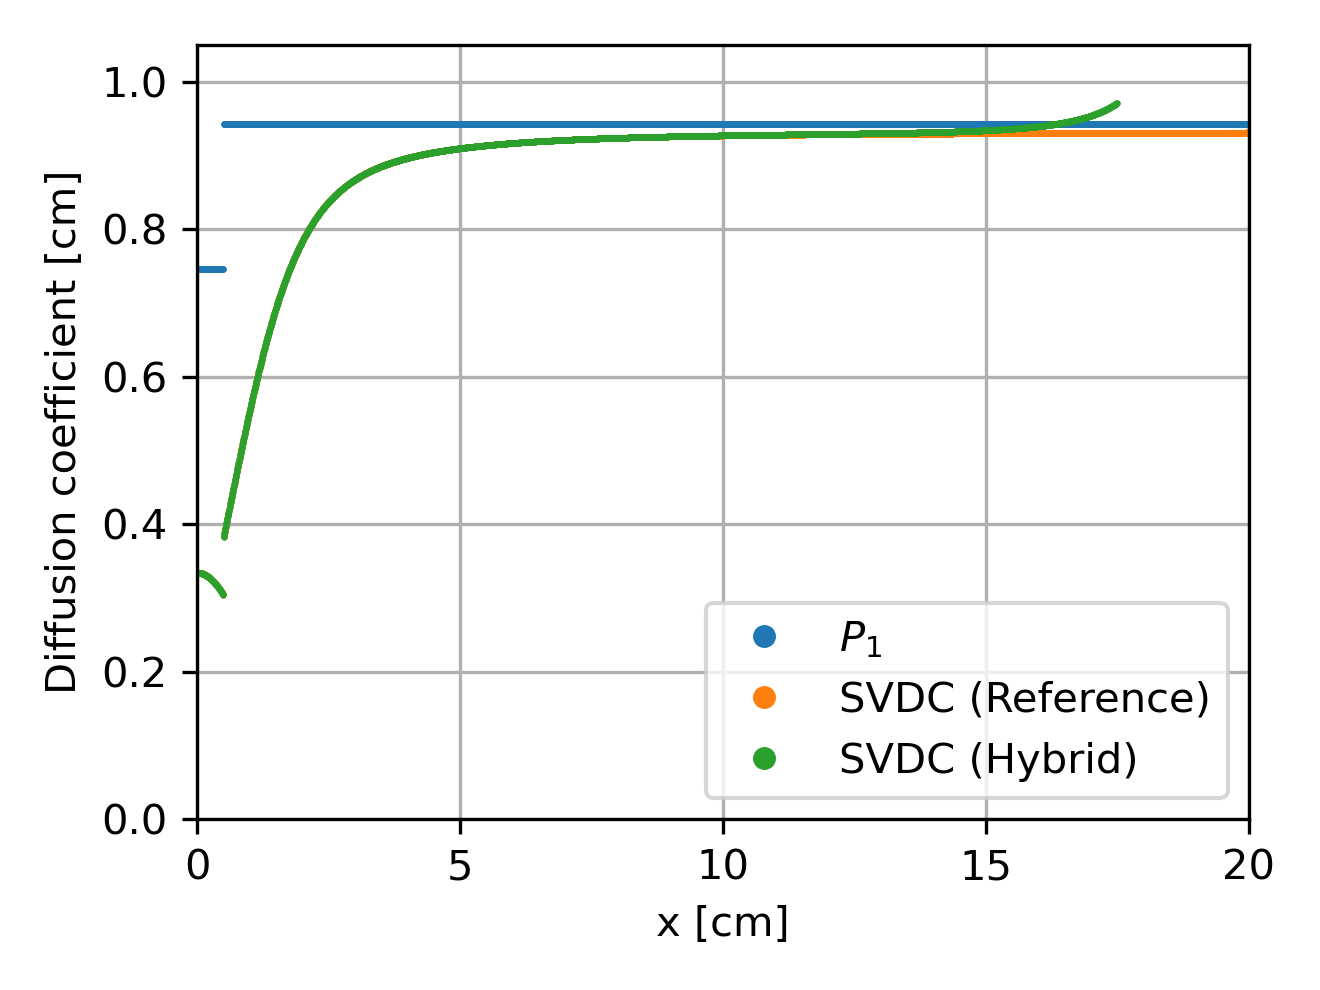
\includegraphics[width=\textwidth]{case-0-group-1-hybrid-diffcoef}
    \caption{Group 1 diffusion coefficients}
    \label{fig:c0g1hd}
  \end{subfigure}
  \hfill
  \begin{subfigure}[b]{.49\textwidth}
    \centering
    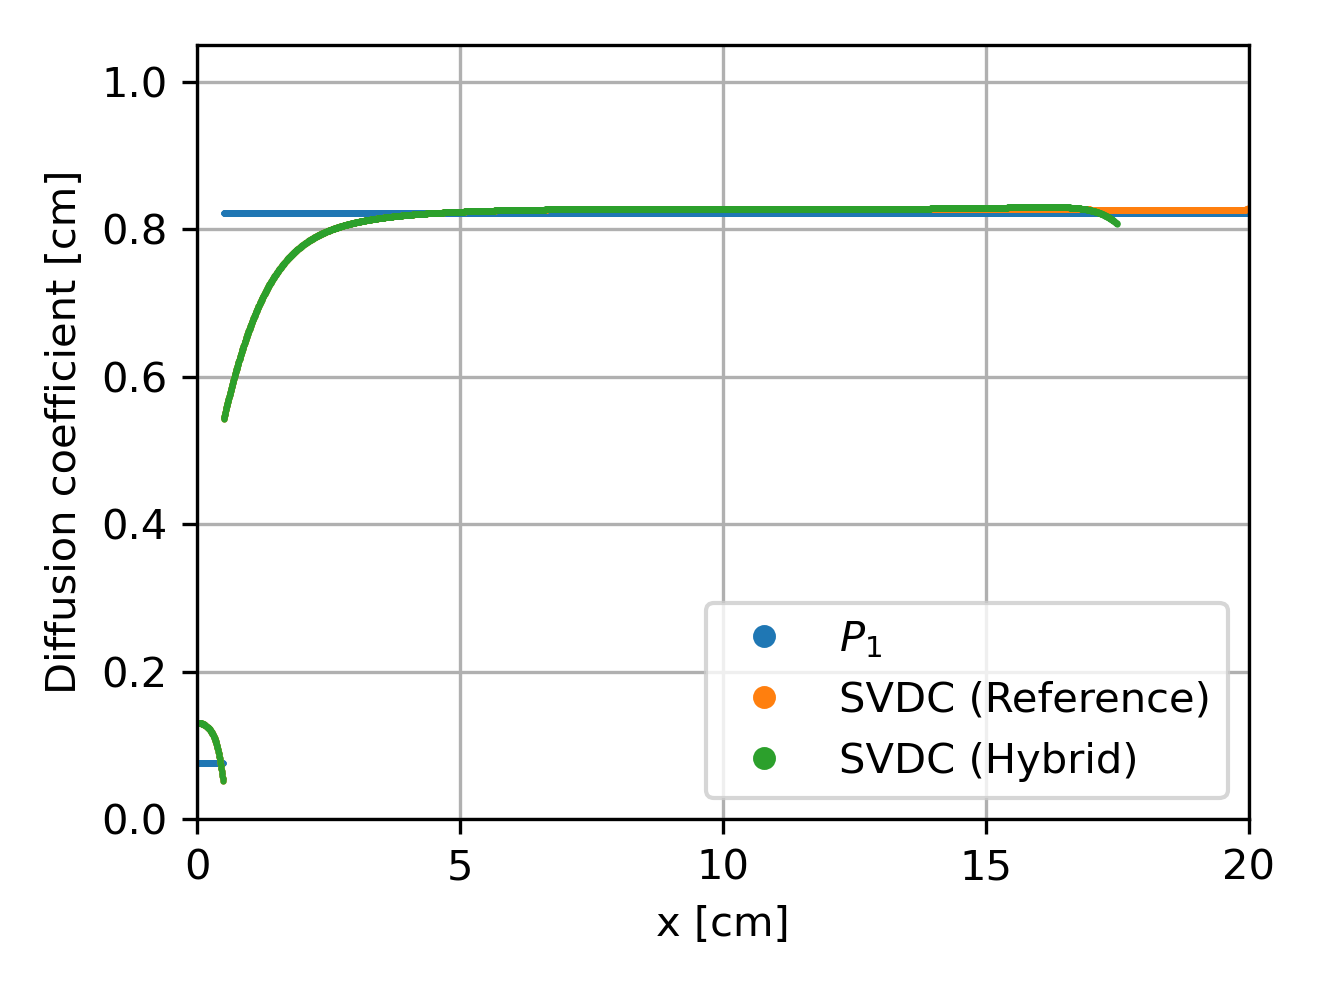
\includegraphics[width=\textwidth]{case-0-group-2-hybrid-diffcoef}
    \caption{Group 2 diffusion coefficients}
    \label{fig:c0g2hd}
  \end{subfigure}
  \caption{$P_1$-based flux-limited diffusion coefficient and \gls{SVDC} spatial distribution for
  Case 0. The \gls{SVDC} distributions were generated from the reference $S_4$ (Full) and the
  hybrid (Hybrid) calculations.}
  \label{fig:c0hd}
\end{figure}

For a visual illustration, refer to Figures \ref{fig:c0g1hd} and \ref{fig:c0g2hd} which plot the
group 1 and 2 $P_1$-based diffusion coefficients, \glspl{SVDC} derived from the reference $S_4$
calculation as demonstrated in Section \ref{sec:svdc}, and \glspl{SVDC} derived from the Hybrid
$S_N$-Diffusion method discussed here. The first set of \glspl{SVDC} are taken to be the reference
because it was generated from a $S_4$ calculation across the entire domain $\Omega^d_0$. The
reference \glspl{SVDC} are labelled ``Full'' in the figures to avoid confusion with the reference
flux distribution from the $S_4$ calculation. The \glspl{SVDC} from the hybrid method agrees well
with the reference \glspl{SVDC} in the control rod region and for most of the fuel-graphite region
up to around $x=12.5$ cm. Both sets of \glspl{SVDC} approximately coincide with the $P_1$ diffusion
coefficient values at $x=14.370$ cm and $x=4.015$ cm for group 1 and group 2, respectively. The
dead zone spans from $x=14.370$ cm to $x=17.500$ cm for group 1 and $x=4.015$ cm to $x=17.500$ cm
for group 2, in which the hybrid method defaults to the $P_1$-based diffusion coefficients by
definition. Given that the reference \glspl{SVDC} values will generally not be known in real-world
problems, the hybrid method relies on the matching of \gls{SVDC} and $P_1$ diffusion coefficient
values for determining the dead zone cutoff point. Another important consideration is the fact that
the neutron flux gradient will be discontinuous if the \gls{SVDC} and $P_1$ diffusion coefficient
values are not sufficiently continuous at the dead zone cutoff point. A flux gradient discontinuity
in a homogeneous bulk region is non-physical and therefore unacceptable. In Section
\ref{sec:prelim-results}, I study \gls{SVDC} distribution trends in more heterogeneous systems and
their implications on determining the dead zone cutoff point.
%
\begin{figure}[htb!]
  \centering
  \begin{subfigure}[b]{.49\textwidth}
    \centering
    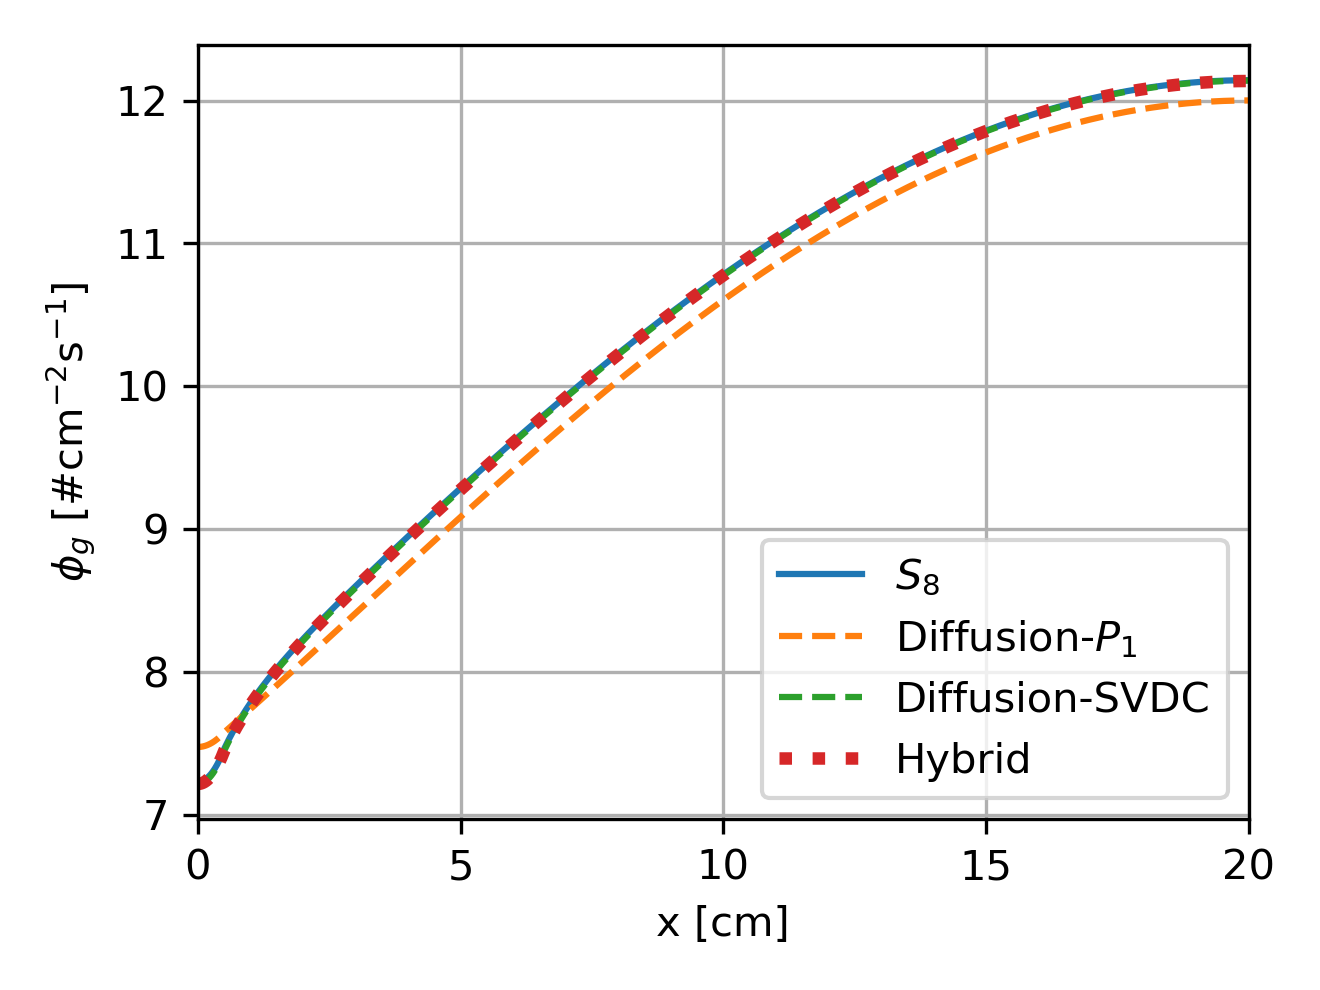
\includegraphics[width=\textwidth]{case-0-group-1-hybrid-flux}
    \caption{Group 1 flux}
    \label{fig:c0g1hf}
  \end{subfigure}
  \hfill
  \begin{subfigure}[b]{.49\textwidth}
    \centering
    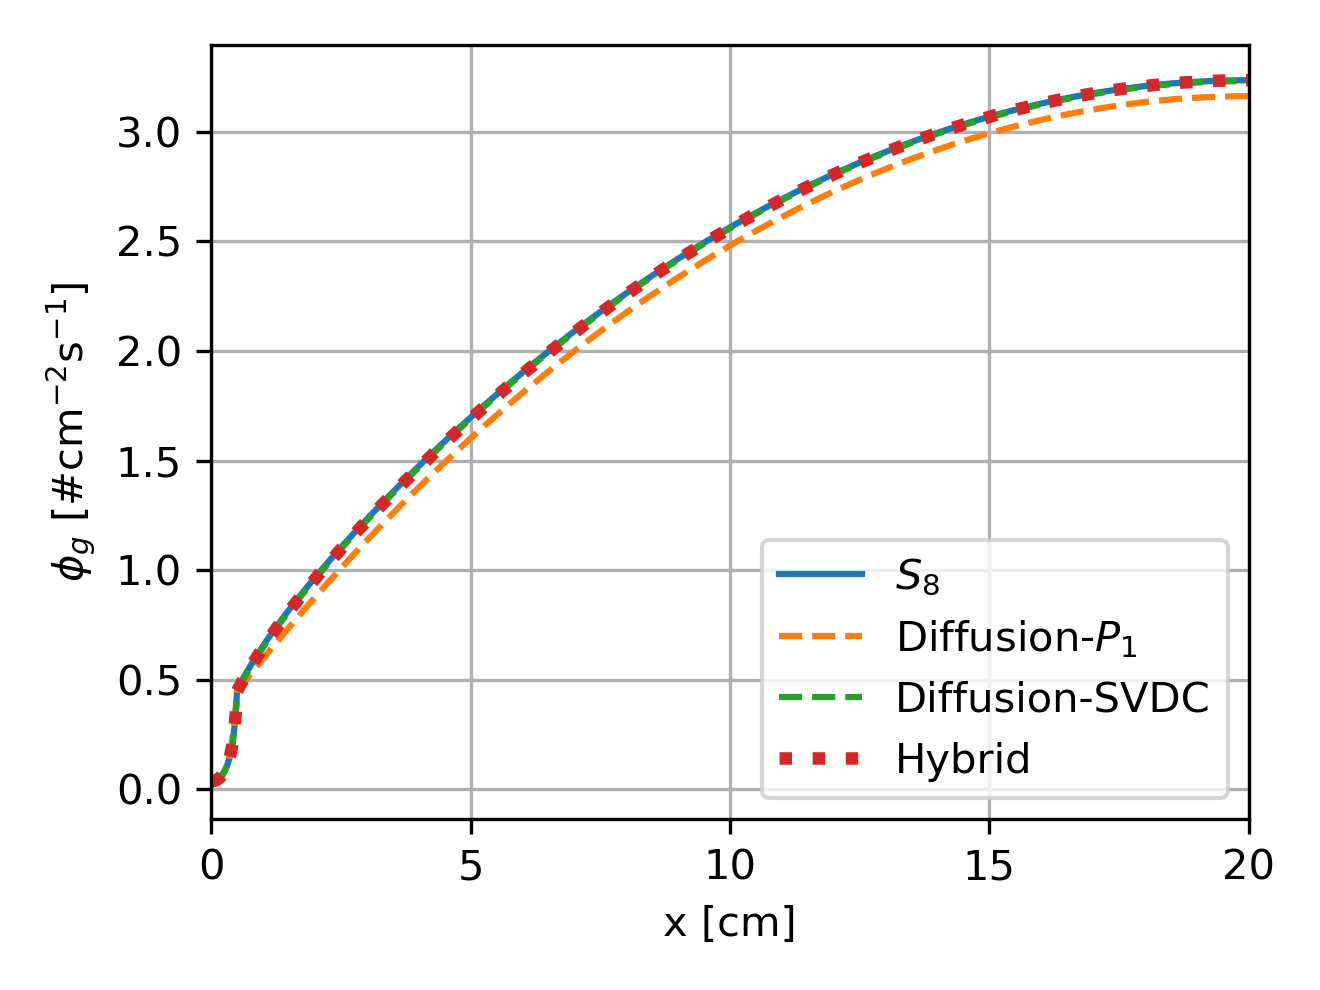
\includegraphics[width=\textwidth]{case-0-group-2-hybrid-flux}
    \caption{Group 2 flux}
    \label{fig:c0g2hf}
  \end{subfigure}
  \caption{Neutron group 1 and 2 flux distributions from the diffusion, $S_4$, reference
  \gls{SVDC}, and hybrid solvers for Case 0.}
  \label{fig:c0hf}
\end{figure}

Figures \ref{fig:c0g1hf} and \ref{fig:c0g2hf} show the group 1 and 2 neutron flux distributions
from the neutron diffusion calculations with $P_1$ diffusion coefficients and \glspl{SVDC}, and
$S_4$ calculation. As expected following the diffusion coefficient discussion, the hybrid method
flux distribution matches the $S_4$ flux distribution well. The $k$ estimate from the hybrid
method is 0.62574 which is only 0.00020 higher than the diffusion calculation with reference
\glspl{SVDC} (0.62554), and 0.00150 higher than the $S_4$ calculation (0.62424). By comparison, the
$k$ estimate from the diffusion calculation with $P_1$ diffusion coefficients is 0.01448 lower than
the $S_4$ calculation as discussed in Section \ref{sec:svdc}.

In Case 0, $\Omega^d_1$ covers more than half of $\Omega^d_0$ due to
the control rod region being the only significant influence on the neutron flux distribution in the
otherwise homogeneous system with reflective boundary conditions. I chose Case 0 as a simple test
case to aid in introducing the Hybrid $S_N$-Diffusion method. In the next section, I
present numerical implementation details of the Hybrid $S_N$-Diffusion method and results on more
complicated geometries with neutron reflector, air, and heterogeneous fuel-graphite lattice
regions and vacuum boundary conditions. On these test cases, the hybrid method yields
smaller $\Omega^d_1$-to-$\Omega^d_0$ ratios than the corresponding ratio in Case 0.

\section{Numerical Implementation} \label{sec:implementation}

I implemented all numerical solvers discussed in this work in the Python programming language.
First, I discuss the material group constant data generation and postprocessing steps. Next, I
present the implementation details of the neutron diffusion and $S_N$ numerical methods
individually. Thereafter I present how they are coupled to form the Hybrid $S_N$-Diffusion method.

\subsection{Group Constant Data Generation}

The group constants required by either or both neutron diffusion and $S_N$ neutron transport
methods are
%
\begin{itemize}
  \item $\Sigma_{t,g}$: Macroscopic total cross section in group $g$
  \item $\Sigma_{r,g}$: Macroscopic removal cross section in group $g$
  \item $\Sigma_s^{g'\rightarrow g}$: Macroscopic group-to-group scattering cross section matrix
  \item $\Sigma_{s,l}^{g'\rightarrow g}$: $l$-th Legendre expansion of the macroscopic
    group-to-group scattering cross section matrix
  \item $\Sigma_{sp,l}^{g'\rightarrow g}$: $l$-th Legendre expansion of the macroscopic
    group-to-group scattering production cross section matrix
  \item $D_g$: $P_1$-based diffusion coefficient in group $g$
  \item $\nu\Sigma_{f,g}$: Product of the average number of neutrons produced per fission and the
    macroscopic fission cross section in group $g$
  \item $\chi_g$: Neutron fission spectrum in group $g$
\end{itemize}
%
These group constants are generated using OpenMC's multigroup cross section generation capability
and postprocessed using a Python script into a JSON file format. $\Sigma_{r,g}$ is the only
quantity that is not directly provided by OpenMC. It is calculated as
%
\begin{align}
  \Sigma_{r,g} =& \sum^G_{g'\neq g}\Sigma_s^{g\rightarrow g'}+\Sigma_{a,g}-\left(\Sigma_{sp}^{g
    \rightarrow g} - \Sigma_s^{g\rightarrow g}\right)
  \shortintertext{where}
      \Sigma_{a,g} =& \mbox{ macroscopic absorption cross section in group $g$,} \nonumber \\
      \Sigma_{sp}^{g\rightarrow g} =& \mbox{ macroscopic scattering production cross section from
      group $g$ to $g$.} \nonumber
\end{align}
%
$\Sigma_{r,g}$ primarily represents the loss of neutrons through outscattering and absorption.
$\Sigma_{sp}^{g\rightarrow g}$ incorporates neutron multiplication effects from neutron knockout
reactions into the scattering cross section. Neutron knockout reactions are commonly tallied as
scattering reactions, and $\Sigma_{r,g}$ is a convenient term through which to incorporate neutron
knockout effects into the neutron diffusion equations.

OpenMC uses the $P_1$ flux-limited formulation \cite{pomraning_flux-limited_1984} for calculating
$D_g$ as follows
%
\begin{align}
  D_g =& \frac{1}{3\Sigma_{tr,g}} \\
  \Sigma_{tr,g} =& \frac{\langle\Sigma_{t,g}\phi_g\rangle-\langle\Sigma_{s1,g}\phi_g\rangle}
  {\langle\phi_g\rangle}
  \shortintertext{where}
  \langle\Sigma_{t,g}\phi_g\rangle =& \int_{r\in V}dr \int_{4\pi}d\Omega\int^{E_{g-1}}_{E_g}dE\
  \Sigma_{t,g}(r,E)\Psi(r,E,\Omega) \nonumber \\
  \langle\Sigma_{s1,g}\phi_g\rangle =& \int_{r\in V}dr \int_{4\pi}d\Omega\int^{E_{g-1}}_{E_g}dE
  \int_{4\pi}d\Omega'\int^{\infty}_0dE'\int^1_{-1}d\mu\ \mu\Sigma_s(r,E'\rightarrow E,\Omega'\cdot
  \Omega)\phi(r,E',\Omega') \nonumber \\
  \langle \phi \rangle =& \int_{r\in V}dr\int_{4\pi}d\Omega\int^{E_{g-1}}_{E_g}dE\ \Psi(r,E,\Omega)
  .\nonumber
\end{align}

\subsection{Neutron Diffusion Method}

On a 1-D uniform spatial grid with $I+1$ mesh points, the neutron scalar flux variables
$\phi_{g,i}$ are defined on the mesh points $x_i$. Theoretically, group constants are volumetric
material properties which should be defined on the cell-centered half-integer mesh points
$x_{i+\sfrac{1}{2}}$. In practice, all material properties except diffusion coefficients are
uniform in each subregion and are sampled at $x_i$. To avoid ambiguity concerning diffusion
coefficient sampling, I formulated all test cases such that all material interfaces fall on $x_i$.
A ghost point is added to the end of the spatial grid if the reflective boundary conditions are
imposed at that boundary.

Discretizing the multigroup time-independent neutron diffusion equations in Eq. \ref{eq:1d-diff}
and reformulating the scattering term using neutron balance in the control volume bounded by
$x_{i-\sfrac{1}{2}}$ and $x_{i+\sfrac{1}{2}}$ yields
%
\begin{align}
  J_{g,i+\sfrac{1}{2}} - J_{g,i-\sfrac{1}{2}} + \Sigma_{t,g,i} \phi_{g,i} \Delta x = \sum^G_{g'=1}\left[
  \Sigma_{s,i}^{g'\rightarrow g}\phi_{g',i} + \chi_{g,i}\frac{\nu\Sigma_{f,g',i}}{k} \phi_{g',i}
\right]\Delta x. \label{eq:diff-j}
\end{align}
%
Using a 1st-order diamond difference scheme to replace the $J$ terms with the discretized form of
Fick's first law of diffusion,
%
\begin{align}
  J_{g,i+\sfrac{1}{2}} = -D_{g,i+\sfrac{1}{2}}\frac{d\phi_{g,i+\sfrac{1}{2}}}{dx} =
  -D_{g,i+\sfrac{1}{2}} \frac{\phi_{g,i+1}-\phi_{g,i}}{\Delta x},
\end{align}
%
and rearranging the terms in Eq. \ref{eq:diff-j} yields
%
\begin{align}
  -\frac{D_{g,i-\sfrac{1}{2}}}{\Delta x} \phi_{g,i-1} + &\left[\frac{D_{g,i-\sfrac{1}{2}}+
  D_{g,i+\sfrac{1}{2}}}{\Delta x} + \Delta x\ \Sigma_{r,g,i} \right]\phi_{g,i} -
  \frac{D_{g,i+\sfrac{1}{2}}}{\Delta x}\phi_{g,i+1} -\Delta x\sum^G_{g'\neq g}
  \Sigma_{s,i}^{g'\rightarrow g}\phi_{g',i} \nonumber \\
  =& \Delta x\sum^G_{g'=1}
  \chi_{g,i} \frac{\nu\Sigma_{f,g',i}}{k} \phi_{g',i}, \label{eq:diff-fd}
  \shortintertext{where}
  \Sigma_{r,g} =& \Sigma_{t,g} - \Sigma_s^{g\rightarrow g} \nonumber \\
  =& \mbox{ macroscopic removal cross section for neutron group }g. \nonumber
\end{align}
%
The fixed neutron source $S_g$ is ignored here since the test cases are all neutron-multiplying
systems with no fixed source.

I implemented two types of boundary conditions: vacuum and reflective boundary conditions. The
\textbf{vacuum boundary conditions} are imposed by setting the incoming flux in the $P_1$
approximation to zero as follows
%
\begin{align}
  \mbox{Left boundary: } \frac{\phi_{g,0}}{4}-\frac{\phi_{g,1}-\phi_{g,0}}{2\Delta x} =& 0 \\
  \mbox{Right boundary: } \frac{\phi_{g,I}}{4}+\frac{\phi_{g,I}-\phi_{g,I-1}}{2\Delta x} =& 0.
\end{align}
%
The \textbf{reflective boundary conditions} are imposed by setting equating the flux at the last physical
mesh point to the flux at the ghost point as follows
%
\begin{align}
  \mbox{Left boundary: } \phi_{g,-1} =& \phi_{g,0} \\
  \mbox{Right boundary: } \phi_{g,I} =& \phi_{g,I+1}
\end{align}
%
where the $-1$ and $I+1$ indexes correspond to ghost point indexes. At material interfaces,
the continuity condition requires that the net neutron current on either side of the interface be
equal as follows
%
\begin{align}
  -D_{g,j-\sfrac{1}{2}}\frac{\phi_{g,j}-\phi_{g,j-1}}{\Delta x} = -D_{g,j+\sfrac{1}{2}}
  \frac{\phi_{g,j+1}-\phi_{g,j}}{\Delta x} \label{eq:itf-bc}
\end{align}
%
for a material interface at $x_j$.

Altogether, they form a system of equations of the form $\bm{A\overline{\phi}}=\bm{\frac{1}{k}
B\overline{\phi}}$, where $\bm{\overline{\phi}}$ is a flattened vector representation of
$\phi_{g,i}$, and $\bm{A}$ and $\bm{B}$ are matrices of the coefficients of $\phi_{g,i}$ as given
by Eqs. \ref{eq:diff-fd} to \ref{eq:itf-bc}. I implemented the inverse power method to find $k$ and
$\overline{\phi}$. The inverse power method algorithm is as follows
%
\begin{align}
  \shortintertext{1. Initialize $k^0$ and $\bm{\overline{\phi}}^0$}
  \shortintertext{2. Update $\bm{\overline{\phi}}$ and $k$}
  \bm{\overline{\phi}}^m =& \frac{1}{k^{m-1}}\bm{A}^{-1}\bm{B\overline{\phi}}^{m-1} \\
  k^m =& k^{m-1}\frac{|\bm{B\overline{\phi}}^m|}{|\bm{B\overline{\phi}}^{m-1}|}
  \shortintertext{3. Check whether convergence is reached}
  \frac{|\bm{\overline{\phi}}^m-\bm{\overline{\phi}}^{m-1}|}{|\bm{\overline{\phi}}^m|} <& \
  tol_{\bm{\overline{\phi}}} \\
  \frac{|k^m-k^{m-1}|}{|k^m|} <& \ tol_k
  \shortintertext{4. Return to Step 2 if either expression is false, otherwise exit.} \nonumber
\end{align}
%
$k^m$ and $\overline{\phi}^m$ denote estimates of $k$ and $\overline{\phi}$ after the $m$-th
iteration. Matrix $\bm{A}$ is a primarily tridiagonal matrix with at most $G-1$ off-diagonal terms
from the 4th term in Eq. \ref{eq:diff-fd}. Thus, $\bm{A}$ is initialized as a sparse matrix to take
advantage of the computationally efficient sparse matrix solver functions from the \texttt{sparse}
class of the \texttt{SciPy} Python library for scientific and technical computing. Matrix $\bm{B}$
is never initialized explicitly as a matrix. Instead, the vector $\bm{b}=\bm{B\overline{\phi}}$ is
updated directly in every iteration. In this system of equations, $|\bm{b}|$ corresponds to the
total number of fission neutrons produced in the system for a given $\bm{\overline{\phi}}$. This
quantity is calculated using the \texttt{trapezoid} numerical integration function from
\texttt{SciPy} to estimate the integral value of $\nu\Sigma_{g,f}\phi_{g}$ in $x$ from the discrete
flux values in $\bm{x}$. Finally, the final $\phi_{g,i}$ is normalized by a factor of $|\bm{b}|/k$
(no. of source neutrons) to obtain the neutron scalar flux per source neutron.

\subsection{$S_N$ Neutron Transport Method}

For the 1-D $S_N$ neutron transport method on the same uniform spatial grid with $I+1$ mesh points,
the neutron angular flux variables $\Psi_{g,i,n}=\Psi_g(x_i,\mu_n)$ are defined on the mesh points
$x_i$ while neutron scalar flux variables $\phi_{g,i\pm\sfrac{1}{2}}$ are defined on the
half-integer mesh points $x_{i\pm\sfrac{1}{2}}$. All group constants are sampled at
$x{i\pm\sfrac{1}{2}}$.

The $S_N$ equations are solved using the transport sweep method in which the algorithm ``sweeps''
through the spatial grid and sequentially updates $\Psi_{g,i,n}$. In 1-D, the algorithm sweep
direction follows the direction of neutron travel, i.e. it sweeps in the positive direction for
$\Psi_{g,i,n}$ with $\mu_n>0$ and vice versa.

Discretizing the multigroup $S_N$ neutron transport equations in Eq. \ref{eq:1d-sn} about
$x_{i+\sfrac{1}{2}}$ yields
%
\begin{align}
  \mu_n\frac{\Psi_{g,i+1,n}-\Psi_{g,i,n}}{x_{i+1}-x_i} + \Sigma_{t,g,i+\sfrac{1}{2}}
  \Psi_{g,i+\sfrac{1}{2},n} = q_{g,i+\sfrac{1}{2},n}
\end{align}
%
where $q_{g,i+\sfrac{1}{2},n}$ represents the combined scattering and fission neutron source term.
After expressing $\Psi_{g,i+\sfrac{1}{2}}$ as the average of $\Psi_{g,i+1,n}$ and $\Psi_{g,i,n}$
in the 1st-order diamond difference scheme and rearranging the terms, we obtain
%
\begin{align}
  \Psi_{g,i+1,n} =& \frac{1-\Sigma_{t,g}\Delta x/2\mu_n}{1+
    \Sigma_{t,g}\Delta x/2\mu_n}\Psi_{g,i,n} +
    q\frac{\Delta x}{\mu_n\left(1+\Sigma_{t,g}\Delta x/2\mu_n\right)} \label{eq:sweep-right} &&
    (\mbox{for } \mu_n > 0)
\shortintertext{and}
  \Psi_{g,i,n} =& \frac{1+\Sigma_{t,g}\Delta x/2\mu_n}{1-
    \Sigma_{t,g}\Delta x/2\mu_n}\Psi_{g,i+1,n} -
    q\frac{\Delta x}{\mu_n\left(1-\Sigma_{t,g}\Delta x/2\mu_n\right)}. \label{eq:sweep-left} &&
    (\mbox{for } \mu_n < 0)
\end{align}
%
The remaining $i+\sfrac{1}{2}$ indexes on the group constants are dropped to reduce visual clutter.
These expressions are used to update $\Psi_{g,i,n}$ in the forward and backward transport sweeps.

The discretized scattering and fission terms in $q_{g,i+\sfrac{1}{2},n}$ are given as
%
\begin{align}
  q_{g,i+\sfrac{1}{2},n} =& \sum^G_{g'=1}\sum^L_{l=0}\frac{\left(2l+1\right)}
  {2}\Sigma_{s,l}^{g'\rightarrow g}P_l(\mu_n)\phi_{l,g',i+\sfrac{1}{2}} \nonumber \\
  &+\frac{\chi_g}{2}\sum^G_{g'=1}\frac{\nu\Sigma_{f,g'}}{k}\phi_{0,g',i+\sfrac{1}{2}}
  \label{eq:sn-q}
  \shortintertext{where}
  \phi_{l,g',i+\sfrac{1}{2}} =& \sum^N_{n'=1}w_{n'}P_l(\mu_{n'})\frac{\Psi_{g',i,n'}+
  \Psi_{g',i+1,n'}}{2}. \label{eq:phi-l}
\end{align}
%
$\phi_{l,g,i}$ are $l$-th Legendre expansions of the neutron flux evaluated using Gauss-Legendre
quadrature over $\mu_{n'}=[-1,1]$. $\phi_{0,g,i}$ and $\phi_{1,g,i}$ also correspond to the neutron
scalar flux $\phi_{g,i}$ and net current $J_{g,i}$, respectively.

For vacuum boundary conditions, $\Psi_{g,0,n}$ is zero for all positive $\mu_n$ while
$\Psi_{g,I,n}$ is zero for all negative $\mu_n$ as follows
%
\begin{align}
  \mbox{Left boundary: } \Psi_{g,0,n} =& 0 && (\mbox{for } \mu_n > 0) \\
  \mbox{Right boundary: } \Psi_{g,I,n} =& 0 && (\mbox{for } \mu_n < 0)
\end{align}
%
Reflective boundary conditions are imposed by equating the incoming angular flux to the
outgoing angular flux in the opposite direction as follows
%
\begin{align}
  \mbox{Left boundary: } \Psi_{g,0,n} =& \Psi_{g,0,n'} && (\mbox{for } \mu_n > 0, \mu_n =
  -\mu_{n'}) \\
  \mbox{Right boundary: } \Psi_{g,I,n} =& \Psi_{g,I,n'} && (\mbox{for } \mu_n < 0, \mu_n =
  -\mu_{n'})
\end{align}

The power iteration algorithm for the $S_N$ method is similar to the inverse power method algorithm
applied in the neutron diffusion method. The matrix solving step for updating $\overline{\phi}$ is
replaced with the transport sweep step along with its associated steps as follows
%
\begin{align}
  \shortintertext{1. Initialize $k^0$, $\phi_{l,g,i+\sfrac{1}{2}}^0$, and $q^0$}
  \shortintertext{2. Apply transport sweeps to solve for $\Psi^m$ using Eqs. \ref{eq:sweep-right},
  \ref{eq:sweep-left}, and \ref{eq:sn-q}}
  \shortintertext{3. Update $\phi^m$ and $k^m$ using Eqs. \ref{eq:phi-l} and \ref{eq:sn-k}}
  k^m =& k^{m-1}\frac{\sum^I_{i=0}\sum^G_{g=1}\nu\Sigma_{f,g}\phi^m_{g,i+\sfrac{1}{2}}}
  {\sum^I_{i=0}\sum^G_{g=1}\nu\Sigma_{f,g}\phi^{m-1}_{g,i+\sfrac{1}{2}}} \label{eq:sn-k}
  \shortintertext{4. Check whether convergence is reached}
  \frac{|\bm{\overline{\phi}}^m-\bm{\overline{\phi}}^{m-1}|}{|\bm{\overline{\phi}}^m|} <& \
  tol_{\bm{\overline{\phi}}} \\
  \frac{|k^m-k^{m-1}|}{|k^m|} <& \ tol_k
  \shortintertext{5. Return to Step 2 if either expression is false, otherwise exit.} \nonumber
\end{align}

The transport sweep and $\phi^m$-update algorithms are parallelized using the \texttt{joblib}
parallel computing Python library across all available CPU threads. The total computational work is
subdivided into several smaller tasks by unique combinations of the $G$ and $N$ indexes; each
thread computes all $\Psi^m$ or $\phi^m$ values on the mesh for a given set of indexes $g$ and
$n$.

\subsection{Hybrid $S_N$-Diffusion Method}



\section{Description of 1-D Models}

\section{Results} \label{sec:prelim-results}

\section{Summary}

The Hybrid $S_N$-Diffusion method is promising for studying reactor systems such as \glspl{MSR},
which consist of mostly highly scattering regions (small neutron mean free path), because the $S_N$
subproblem domain $\Omega^d_1$ covers a small fraction of the entire reactor geometry. This
reduces the computational costs of the iterative $S_N$ calculations in the hybrid method.
